\documentclass{beamer}
\usepackage{amsmath,amssymb,latexsym,array,fancyheadings,mathdots}
\usepackage{algorithm,algorithmic}
\usepackage{hyperref}
\usepackage{color}
\usepackage{tabularx}
\usepackage[all]{xy}
\usepackage{qtree}
\usepackage{gitinfo2}

%% RCS
%\usepackage{rcs}

%% Colors
\definecolor{darkgreen}{rgb}{0,.4,0}
\definecolor{darkred}{rgb}{.5,0,0}
\definecolor{darkmagenta}{rgb}{.5,0,.5}
\definecolor{orange}{rgb}{1,.5,0}
\definecolor{lightblue}{rgb}{0.122,0.016,0.855}
\definecolor{darkocre}{rgb}{0.471,0.298,0.008}

\usetheme{default}

%% New Theorems
\newtheorem{thm}{Theorem}
\newtheorem{exm}[thm]{Example}
\newtheorem{cor}[thm]{Corollary}
\newtheorem{propo}[thm]{Proposition}
\newtheorem{lem}[thm]{Lemma}
\newtheorem{clm}[thm]{Claim}
\newtheorem{exr}[thm]{Exercise}
\newtheorem{dfn}[thm]{Definition}

%% New commands
\newcommand{\classfont}{\mathsf}
\newcommand{\ATM}{\classfont{A}_{\mathrm{TM}}}
\newcommand{\MTF}{\mathrm{MTF}}
\newcommand{\OPT}{\mathrm{OPT}}
\newcommand{\ALG}{\mathrm{ALG}}
\newcommand{\ALGNAIVE}{\mathrm{ALG}_{\text{na{\"\i}ve}}}
\newcommand{\LRU}{\mathrm{LRU}}
\newcommand{\FIFO}{\mathrm{FIFO}}
\newcommand{\FWF}{\mathrm{FWF}}
\newcommand{\LFD}{\mathrm{LFD}}
\newcommand{\true}{\mathsf{T}}
\newcommand{\false}{\mathsf{F}}
\newcommand{\also}{\wedge}
\newcommand{\lra}{\leftrightarrow}
\newcommand{\tc}{\textcolor}
\newcommand{\df}[1]{\textcolor{red}{\em #1}}
\newcommand{\highlight}[1]{\textcolor{orange}{\em #1}}
\newcommand{\hl}[1]{\textcolor{blue}{\em #1}}
\newcommand{\amp}{\texttt{\&}}
\newcommand{\hsh}{\texttt{\#}}
\newcommand{\ra}{\rightarrow}
\newcommand{\longra}{\longrightarrow}
\newcommand{\Ra}{\Rightarrow}
\newcommand{\rab}{{\rightarrow_\beta}}
\newcommand{\srab}{{\rightarrow^*_\beta}}
\newcommand{\aeq}{{=_\alpha}}
\newcommand{\order}{\mathrm{order}}
\newcommand{\rem}{\mathrm{rem}}
\newcommand{\IP}{\mathbf{IP}}
\newcommand{\PSPACE}{\mathbf{PSPACE}}
\newcommand{\thevalue}{\text{value}}
\newcommand{\pol}[1]{\mathbf{#1}}
\newcommand{\enc}{\text{Enc}}
\newcommand{\xor}{\oplus}
\newcommand{\zo}{\{0,1\}}
\newcommand{\SOPT}{S_{\mathrm{opt}}}
\newcommand{\la}{\leftarrow}
\newcommand{\myurl}[1]{\textcolor{darkgreen}{\url{#1}}}
\newcommand{\myhref}[2]{\textcolor{darkgreen}{\href{#1}{#2}}}
\newcommand{\qaccept}{q_{\mathrm{accept}}}
\newcommand{\qreject}{q_{\mathrm{reject}}}
\newcommand{\opt}{\text{\sc Opt}}
\newcommand{\tr}{\mathrm{tr}}
\newcommand{\csanky}{p^{\textsc{csanky}}}
\newcommand{\berk}{p^{\textsc{berk}}}

%% Algorithms package customization
\renewcommand{\algorithmicrequire}{\textbf{Pre-condition:}} 
\renewcommand{\algorithmicensure}{\textbf{Post-condition:}} 
\algsetup{indent=3em}

\input{prooftree}

%% including/excluding pauses
\newcommand{\ifpause}{\iftrue} % for including pauses
%\newcommand{\ifpause}{\iffalse} % for excluding pauses

%% 2nd or 3rd edition
\newif\ifthird
\thirdtrue
%\thirdfalse

%disables usefoottemplate
\setbeamertemplate{navigation symbols}{}
%\setbeamertemplate{footline}% 
%{\strut\quad\tiny 
%\begin{minipage}{3cm}
%Cryptography - Michael Soltys
%\today\ {\tt v\RCSRevision}
%\end{minipage}\hfill
%\insertsection\
%- \insertframenumber/\inserttotalframenumber\quad\strut}

\newcommand{\mytitle}{Divide \&\ Conquer}
\newcommand{\mychpnr}{3}
%% Title page contents
\title{Intro to Analysis of Algorithms \\ \mytitle \\  Chapter \mychpnr}
\author{Michael Soltys}
\date{\textcolor{darkgreen}{\tiny\tt 
[ {\bf Git} Date:\gitAuthorDate\ 
Hash:\gitAbbrevHash\ 
Ed:\ifthird
3rd
\else
2nd
\fi]}}
\institute{CSU Channel Islands}

\setbeamertemplate{footline}{
  \colorbox{white}{\color{black}\tt
     \begin{tabularx}{0.97\textwidth}{XXX}
          IAA Chp \mychpnr\ - Michael Soltys \copyright & 
          \hfill\today\ (\gitAbbrevHash; \ifthird ed3\else ed2\fi)
					\hfill\phantom{.} & 
          \hfill\insertsection\ - \insertframenumber/\inserttotalframenumber \\
      \end{tabularx}}}

\begin{document}

\mode<presentation>
{
}

\parskip 8pt

\section{Introduction}

\begin{frame}
\titlepage
\end{frame}


\section{Mergesort}

\begin{frame}
\begin{center}
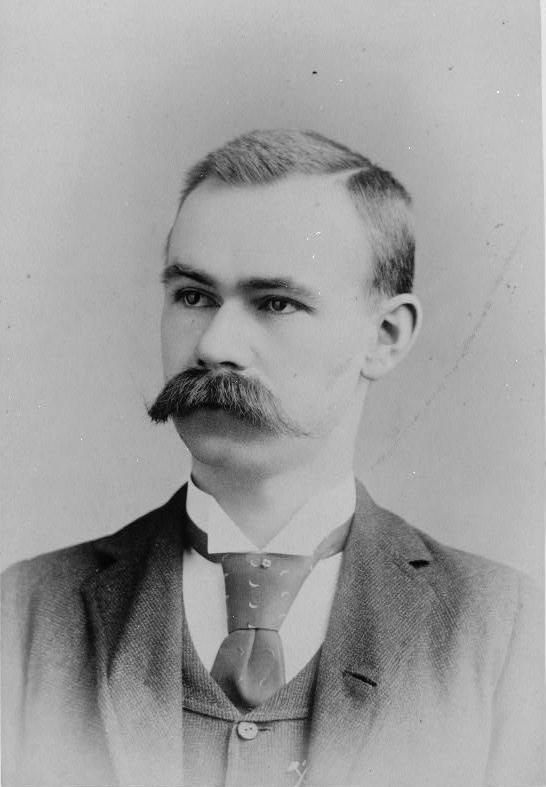
\includegraphics[width=4cm]{Figures/HollerithPhoto.jpg} \\
Herman Hollerith, 1860--1929
\end{center}
\end{frame}

\begin{frame}
Suppose that we have two lists of numbers that are already sorted.

That is, we have a list $a_1\le a_2\le\cdots\le a_n$ and $b_1\le
b_2\le\cdots\le b_m$.  

We want to combine those two lists into one
long sorted list $c_1\le c_2\le\cdots\le c_{n+m}$.

The mergesort algorithm sorts a given list of numbers by first
dividing them into two lists of length $\lceil n/2\rceil$ and $\lfloor
n/2\rfloor$, respectively, then sorting each list recursively, and
finally combining the results.
\end{frame}

\begin{frame}
\begin{algorithmic}[1]
\REQUIRE $a_1\le a_2\le\cdots\le a_n$ and $b_1\le b_2\le\cdots\le b_m$
\STATE $p_1\longleftarrow 1$; $p_2\longleftarrow 1$; $i\longleftarrow 1$
\WHILE{$i\le n+m$}
	\IF{$a_{p_1}\le b_{p_2}$}
		\STATE $c_i\longleftarrow a_{p_1}$
		\STATE $p_1\longleftarrow p_1+1$
	\ELSE
		\STATE $c_i\longleftarrow b_{p_1}$
		\STATE $p_2\longleftarrow p_2+1$
	\ENDIF
	\STATE $i\longleftarrow i+1$
\ENDWHILE
\ENSURE $c_1\le c_2\le\cdots\le c_{n+m}$
\end{algorithmic}
\end{frame}

\begin{frame}
\begin{algorithmic}[1]
\REQUIRE A list of integers $a_1,a_2,\ldots,a_n$
\STATE $L\longleftarrow a_1,a_2,\ldots,a_n$
\IF{$|L|\le 1$}
	\RETURN $L$
\ELSE
	\STATE $L_1\longleftarrow$ first $\lceil n/2\rceil$ elements of $L$
	\STATE $L_2\longleftarrow$ last $\lfloor n/2\rfloor$ elements of $L$
	\RETURN $\text{Merge}(\text{Mergesort}(L_1),\text{Mergesort}(L_2))$
\ENDIF
\ENSURE $a_{i_1}\le a_{i_2}\le\cdots\le a_{i_n}$
\end{algorithmic}
\end{frame}

\begin{frame}
\begin{center}

\includegraphics[width=4cm]{Figures/pearls.png}
\end{center}
\end{frame}

\section{Multiplying nrs in binary}

\begin{frame}
{Multiplication}

\begin{center}
\begin{tabular}{r|cccccccc}
       & 1 & 2 & 3 & 4 & 5 & 6 & 7 & 8    \\\hline
$x$    & &   &   &   & 1 & 1 & 1 & 0       \\
$y$    & &   &   &   & 1 & 1 & 0 & 1       \\\hline
$s_1$  & &   &   &   & 1 & 1 & 1 & 0       \\
$s_2$  & &   &   & 0 & 0 & 0 & 0 &         \\
$s_3$  & &   & 1 & 1 & 1 & 0 &   &         \\
$s_4$  & & 1 & 1 & 1 & 0 &   &   &         \\\hline
$x\times y$ & 1 & 0 & 1 & 1 & 0 & 1 & 1 & 0
\end{tabular}

Multiply $1110$ times $1101$, i.e., $14$ times
$13$.  Takes $O(n^2)$ steps.
\end{center}
\end{frame}

\begin{frame}
{Clever multiplication}

Let $x$ and $y$ be two $n$-bit integers.  We break them up into two
smaller $n/2$-bit integers as follows:
\begin{align*}
x &= (x_1\cdot 2^{n/2}+x_0), \\
y &= (y_1\cdot 2^{n/2}+y_0).
\end{align*}
$x_1$ and $y_1$ correspond to the high-order bits of $x$ and $y$,
respectively, and $x_0$ and $y_0$ to the low-order bits of $x$ and
$y$, respectively.  
\end{frame}

\begin{frame}
The product of $x$ and $y$ appears as follows in
terms of those parts:
\begin{align}
xy &= (x_1\cdot 2^{n/2}+x_0)(y_1\cdot 2^{n/2}+y_0) \tag*{} \\
   &= x_1y_1\cdot 2^n+(x_1y_0+x_0y_1)\cdot 2^{n/2}+x_0y_0\label{eq:recmult}.
\end{align}
A divide and conquer procedure appears surreptitiously.  To compute
the product of $x$ and $y$ we compute the four products
$x_1y_1,x_1y_0,x_0y_1,x_0y_0$, {\em recursively}, and then we combine
them to obtain $xy$.
\end{frame}

\begin{frame}
Let $T(n)$ be the number of operations that are required to compute the
product of two $n$-bit integers using the divide and conquer
procedure:
\begin{equation}\label{eq:rec}
T(n)\le 4T(n/2)+cn,
\end{equation}
since we have to compute the four products
$x_1y_1,x_1y_0,x_0y_1,x_0y_0$ (this is where the $4T(n/2)$ factor
comes from), and then we have to perform three additions of $n$-bit
integers (that is where the factor $cn$, where $c$ is some constant,
comes from).  

Notice that we do not take into account the product by
$2^n$ and $2^{n/2}$ as they simply consist in
shifting the binary string by an appropriate number of bits to the
left ($n$ for $2^n$ and $n/2$ for $2^{n/2}$).  These shift operations
are inexpensive, and can be ignored in the complexity analysis.
\end{frame}

\begin{frame}
It appears that we have to make four recursive
calls; that is, we need to compute the four multiplications
$x_1y_1,x_1y_0,x_0y_1,x_0y_0$.  

But we can get away with only
three multiplications, and hence three recursive calls: $x_1y_1,x_0y_0$
and $(x_1+x_0)(y_1+y_0)$; the reason being that
\begin{equation}\label{eq:recmult2}
(x_1y_0+x_0y_1)=(x_1+x_0)(y_1+y_0)-(x_1y_1+x_0y_0).
\end{equation}
\end{frame}

\begin{frame}
\begin{center}
\begin{tabular}{l|ccc}
                           & multiplications & additions & shifts \\\hline
Method~1 & 4               & 3         & 2      \\
Method~2 & 3               & 4         & 2
\end{tabular}
\end{center}

Algorithm takes $T(n)\le 3T(n/2)+dn$
operations.  

Thus, the running time is $O(n^{\log 3})\approx
O(n^{1.59})$.
\end{frame}

\begin{frame}
{Recursive Binary Mult A\ifthird 3.3\else 3.3\fi}

\begin{algorithmic}[1]
\REQUIRE Two $n$-bit integers $x$ and $y$
\IF{$n=1$}
	\IF{$x=1\wedge y=1$}
		\RETURN $1$
	\ELSE
		\RETURN $0$
	\ENDIF
\ENDIF
\STATE $(x_1,x_0)\longleftarrow$ (first $\lfloor n/2\rfloor$ bits,
																 last $\lceil n/2\rceil$ bits) of $x$
\STATE $(y_1,y_0)\longleftarrow$ (first $\lfloor n/2\rfloor$ bits,
																 last $\lceil n/2\rceil$ bits) of $y$
\STATE $z_1\longleftarrow \mathrm{Multiply}(x_1+x_0,y_1+y_0)$
\STATE $z_2\longleftarrow \mathrm{Multiply}(x_1,y_1)$
\STATE $z_3\longleftarrow \mathrm{Multiply}(x_0,y_0)$
\RETURN $z_2\cdot 2^n+(z_1-z_2-z_3)\cdot 2^{\lceil n/2\rceil}+z_3$
\end{algorithmic}

\end{frame}

\section{Savitch's Algorithm}

\begin{frame}
{\bf Savitch's Algorithm}

We have a directed graph, and we want to establish whether we have a
path from $s$ to $t$.

Savitch's algorithm solves the problem in \df{space} $O(\log^2m)$.

\begin{equation}\label{eq:savitch}
\text{R}(G,u,v,i)\iff
(\exists w)[\text{R}(G,u,w,i-1)\wedge\text{R}(G,w,v,i-1)].
\end{equation}
\end{frame}

\begin{frame}
\begin{algorithmic}[1]
\IF{$i=0$}
	\IF{$u=v$}
		\RETURN $\true$
     	\ELSIF{$(u,v)$ is an edge}
		\RETURN $\true$
	\ENDIF
\ELSE 
	\FOR{every vertex $w$}
    		\IF{$\text{R}(G,u,w,i-1)$ and $\text{R}(G,w,v,i-1)$} 
			\RETURN $\true$
		\ENDIF
	\ENDFOR
\ENDIF
\RETURN $\false$
\end{algorithmic}
\end{frame}

\begin{frame}
{Example run}

\xymatrix{\bullet^1\ar@{-}[r]&\bullet^2\ar@{-}[r]&\bullet^3\ar@{-}[r]&\bullet^4}

Then the recursion stack would look as follows for the first 6 steps:
$$
\begin{array}{c|c|c|c|c|c}
				 &          & R(1,4,0) &    F     & R(2,4,0) &    F     \\
				 &          & R(1,1,0) &    T     & R(1,2,0) &    T     \\
				 & R(1,4,1) & R(1,4,1) & R(1,4,1) & R(1,4,1) & R(1,4,1) \\
         & R(1,1,1) & R(1,1,1) & R(1,1,1) & R(1,1,1) & R(1,1,1) \\
R(1,4,2) & R(1,4,2) & R(1,4,2) & R(1,4,2) & R(1,4,2) & R(1,4,2) \\\hline
\mathrm{Step\ 1} & \mathrm{Step\ 2} & \mathrm{Step\ 3} & \mathrm{Step\ 4} 
& \mathrm{Step\ 5} & \mathrm{Step\ 6} 
\end{array}
$$
\end{frame}

\begin{frame}[fragile]\frametitle{Quicksort \&\ git bisect}

\begin{verbatim}
qsort [] = []
qsort (x:xs) = qsort smaller ++ [x] ++ qsort larger
  where
    smaller = [a | a <- xs, a <= x]
    larger = [b | b <- xs, b > x]
\end{verbatim}
\end{frame}

\end{document}
